\documentclass[sigconf, nonacm, screen]{acmart}

\setlength{\textfloatsep}{8pt plus 2pt minus 2pt}
\setlength{\intextsep}{8pt plus 2pt minus 2pt}

% Drop ACM ConferenceInfo placeholder for non-ACM preprint builds.
\setcopyright{none}
\settopmatter{printacmref=false, printfolios=true}

\usepackage{tikz}
\usetikzlibrary{positioning, arrows, shapes.geometric, fit, backgrounds, calc}
\tikzset{>=stealth}

\usepackage{enumitem}

% acmart sigconf defaults to \flushbottom, which stretches vertical glue
% between section/paragraph breaks to align both columns at the bottom.
% On pages where the content does not naturally fill both columns (e.g.
% page 1 with §1.1 -> §1.2 in the right column), the stretched glue
% appears as ~5 lines of empty space between §1.1's end and §1.2's
% heading. Switching to \raggedbottom suppresses the stretch: columns
% may end ragged but the inter-section gap collapses to the natural
% \subsection space-before (~8 pt).
\raggedbottom

% CONTENT GUIDANCE (delete before submission):
% - One paragraph, 150-250 words.
% - Lead with the problem (memory fragmentation in hybrid Mamba-Transformer
%   serving), the core idea (asymmetric virtual paging with dynamic
%   capacity rebalancing), and the headline result (cross-workload OOM
%   reduction vs the strongest static baseline, see
%   tables/generated/table_baseline_comparison.tex once generated).
% - Do not cite from the abstract; reserve citations for the body.

\begin{abstract}
Hybrid Mamba-Transformer language models combine attention with State Space Models (SSMs), creating asymmetric memory pressure between linearly scaling Key-Value (KV) blocks and fixed-size SSM states. Existing allocator designs for hybrid models typically either pad SSM state into KV-like pages or statically partition memory, which can waste capacity or fail to adapt under shifting workload distributions. Unified pools pad SSM states to match KV pages, causing severe capacity overestimation, while static dual-pool partitions cannot adapt to shifting prompt distributions. We present Asymmetric Virtual Memory Paging (AVMP), a memory allocator that decouples virtual address spaces across physically heterogeneous pools and dynamically rebalances capacity at runtime. We evaluate AVMP across a strictly deterministic 270-cell synthetic sweep plus a 60-cell ShareGPT-Vicuna trace replay, with paired-bootstrap 95\% confidence intervals on every headline claim. The dynamic AVMP allocator records goodput improvements from $1.83\times$ to $13.3\times$ on three synthetic workloads (CIs $[1.42, 2.60]$ to $[11.2, 16.0]$) and $2.36\times$ on ShareGPT (CI $[1.33, 5.65]$), plus a 7.6\% cross-workload Out-of-Memory (OOM) reduction (CI $[3.0\%, 12.7\%]$) against the best static baseline. A wall-clock phase decomposition shows the speedup splits into two mechanisms: faster OOM recovery on workloads with capacity pressure and faster per-call allocator service on workloads without it. Our logical operation counter guarantees byte-identical reproducibility for event-deterministic fields across reruns. We scope this design study as a pure Python prototype evaluated on a single GPU.
\end{abstract}


\begin{document}
\sloppy

\title{Asymmetric Virtual Memory Paging for Hybrid Mamba-Transformer Inference}
\thanks{Source code: \url{https://github.com/codepawl/cachepawl}}

\author{An Xuan Nguyen}
\orcid{0009-0005-6867-1606}
\affiliation{%
  \institution{Codepawl}
  \city{Ho Chi Minh City}
  \country{Vietnam}
}
\email{nxan2911@gmail.com}

\maketitle

\section{Introduction}
\label{sec:intro}

\subsection{Motivation}
\label{sec:intro:motivation}

Recent advancements in large language models extend context length through hybrid architectures. Models like Jamba combine transformer attention mechanisms with State Space Models (SSMs) to support a 256K context window \cite{lieber2024jamba}. The base Jamba architecture also uses a Mixture-of-Experts (MoE) feedforward configuration, though our work focuses specifically on memory management for the attention and SSM cache types; MoE routing memory is orthogonal to this design. This architecture merges two different layer types: attention mechanisms requiring a linearly scaling Key-Value (KV) cache ($O(n)$ per token), and SSMs requiring a fixed-size state footprint ($O(1)$ per layer) \cite{dao2024mamba2}.

Existing inference engines struggle to serve these heterogeneous memory profiles. The unified pool approach in vLLM \cite{kwon2023pagedattention} forces the fixed SSM state to pad up to the attention page size, causing severe capacity overestimation documented in vLLM issue \#37121 (concrete magnitudes in \S\ref{sec:method:avpt}). Alternatively, SGLang implements a static dual pool where operators fix a \texttt{mamba\_full\_memory\_ratio} parameter at engine initialization \cite{zheng2024sglang}. This rigid partition cannot rebalance without a full process restart.

Neither architectural approach handles workload shifts dynamically. Static defaults perform poorly when prompt distributions change during execution. Testing the same workload mix records 1221 Out-of-Memory (OOM) events at a 0.9 static ratio compared to 552 OOMs at a 0.5 static ratio. No existing system provides both asymmetric cache types and runtime adaptivity.

In this paper, we introduce Asymmetric Virtual Memory Paging (AVMP), a paged memory allocator designed specifically for hybrid architectures. AVMP provisions physically asymmetric backing stores while enabling dynamic capacity rebalancing at runtime. Our dynamic rebalancing records a 13.3$\times$ goodput improvement on \texttt{uniform\_short} workloads compared to the best static baseline.

\subsection{Contributions}
\label{sec:intro:contributions}

We make the following specific contributions:

\begin{itemize}[leftmargin=1.4em, itemsep=2pt, topsep=4pt]
\item \textbf{Asymmetric Virtual Page Table Abstraction (\S\ref{sec:method}):} We design a unified virtual handle space spanning two physically heterogeneous backing stores (KV pages and SSM blocks). AVMP extends the GPU virtual memory approach pioneered for KV caches \cite{xu2024vtensor} to two asymmetric pool types. We show that this abstraction introduces no measurable effect on simulated capacity outcomes, with byte-identical OOM counts against a static dual-pool baseline (552 OOMs).

\item \textbf{Dynamic Pool Rebalancing Mechanism (\S\ref{sec:method}):} We implement a \texttt{CapacityError}-triggered migration mechanism that transfers batched memory capacity between pools. We enforce determinism using a logical operation counter rather than wall-clock time, ensuring per-cell byte-identical reproducibility across all experimental reruns.

\item \textbf{Empirical Validation on Hybrid Architectures (\S\ref{sec:eval}):} We execute a 270-cell sweep evaluating 5 allocator variants, 3 synthetic workloads, 3 pool sizes, and 3 random seeds. The dynamic AVMP allocator records a 7.6\% OOM reduction (510 versus 552) against the best static baseline. AVMP records 13.3$\times$ higher goodput on \texttt{uniform\_short}, 2.39$\times$ on \texttt{mixed\_long}, and 1.83$\times$ on \texttt{agentic\_burst} traffic patterns. A parameter sensitivity analysis proves \texttt{migration\_batch\_size} acts as the dominant configuration axis, while a Stage 2 threshold sweep returned a strict null result.

\item \textbf{Open-Source Prototype:} We provide a reference Python implementation and synthetic workload harness with committed sweep artifacts at \url{https://github.com/codepawl/cachepawl}.
\end{itemize}

\section{Background}
\label{sec:background}

% CONTENT GUIDANCE (delete before submission):
% - Subsection 2.1: KV cache in Transformer serving. PagedAttention is
%   the obvious citation (\cite{kwon2023pagedattention}); vLLM-style
%   block-based allocation. Optional: FlashAttention's IO-awareness
%   framing (\cite{dao2023flashattention2}, \cite{shah2024flashattention3}).
% - Subsection 2.2: SSM state caching. The d_state alignment and
%   per-layer constant-size cache shape, contrasted with the KV cache's
%   per-token shape. Cite Mamba (\cite{gu2023mamba}, \cite{dao2024mamba2}).
% - Subsection 2.3: hybrid architectures. Jamba (\cite{lieber2024jamba}),
%   Zamba2 (\cite{glorioso2024zamba2}), Samba (\cite{ren2024samba}),
%   Hymba (\cite{dong2024hymba}), RecurrentGemma
%   (\cite{botev2024recurrentgemma}). Note that none of them prescribe a
%   serving-time memory-layout strategy.
% - Source: RFC 0001 sections 2 and 3.1.

\subsection{Hybrid Mamba-Transformer Architectures}
\label{sec:background:hybrid}

Standard transformer attention requires $O(n^2)$ compute for a sequence of length $n$, and the KV cache grows linearly with $n$ during decoding. Conversely, State Space Models (SSMs) like Mamba operate with $O(n)$ compute and require an $O(1)$ cache per layer \cite{gu2023mamba, dao2024mamba2}. The SSM state size remains fixed and strictly independent of the sequence length. Hybrid architectures combine these two approaches to combine SSM efficiency with attention reasoning.

For example, Jamba mixes attention and Mamba layers at a 1:7 ratio, supporting a 256K token context window with approximately 12B active parameters in a Mixture-of-Experts (MoE) configuration \cite{lieber2024jamba}. Other variations adopt similar hybrid structures with different attention-to-SSM ratios \cite{glorioso2024zamba2, ren2024samba, dong2024hymba, botev2024recurrentgemma}. This architectural combination forces inference engines to manage two fundamentally different memory cache types within a single model.

\subsection{KV Cache and SSM State Management}
\label{sec:background:cache}

Standard transformer inference manages the Key-Value (KV) cache using paged memory allocation \cite{kwon2023pagedattention}, often combined with IO-aware attention kernels \cite{dao2022flashattention, shah2024flashattention3}. The KV cache requires a system that handles variable block sizes, supports append-only operations during decoding, and allows dynamic eviction or recomputation when memory pressure increases. In contrast, the SSM state maintains a fixed size per layer, strictly defined by \texttt{state\_dim} multiplied by \texttt{bytes\_per\_element}. This state updates in place and persists across tokens.

Unlike KV blocks, the SSM state cannot be paged because it lacks a temporal token structure to evict \cite{dao2024mamba2}. It requires a single, contiguous allocation per layer per sequence. Consequently, the memory access patterns diverge significantly: KV cache operations rely on paged scatter-gather memory lookups, while SSM state operations require contiguous read and write access. This structural asymmetry is the root cause of fragmentation and overestimation in existing cache pool designs.

\subsection{Limits of Existing Pool Designs}
\label{sec:background:pool}

Current inference systems attempt to manage hybrid models using either unified or static dual-pool designs, both of which fail in two ways. Unified pools, such as the vLLM \texttt{HybridKVCacheCoordinator} approach \cite{kwon2023pagedattention}, force the SSM state to pad up to the attention page size. As reported in vLLM issue \#37121, this padding causes a 7.3$\times$ KV cache capacity overestimation on Qwen3.5-4B-AWQ, leaving 13.7\% effective VRAM utilization at peak memory. The root cause is the system capacity estimator, which incorrectly multiplies the $O(1)$ SSM state by the sequence token count.

Alternatively, static dual-pool architectures like SGLang pre-allocate two physical regions (\texttt{HybridReqToTokenPool} and \texttt{HybridLinearKVPool}) at engine startup \cite{zheng2024sglang}. This design assigns memory using a fixed parameter, such as a \texttt{mamba\_full\_memory\_ratio} defaulting to 0.9. The system cannot rebalance capacity between pools without a full process restart. When the prompt distribution shifts, static pools perform poorly. As we demonstrate in \S\ref{sec:eval}, a default 0.9 ratio triggers 1221 OOM events compared to 552 OOMs at a 0.5 ratio on identical workloads. Neither unified padding nor static allocation handles runtime workload shifts dynamically, motivating a memory management system that simultaneously supports asymmetric cache types and adapts to shifting prompt distributions.

\section{Method}
\label{sec:method}

% CONTENT GUIDANCE (delete before submission):
% - Subsection 3.1: paraphrase RFC 0001 sections 3-4 (AVMP core design).
%   Source: docs/designs/0001-asymmetric-virtual-memory-paging.md.
% - Subsection 3.2: paraphrase RFC 0002 sections 3-5 (dynamic rebalancing).
%   Source: docs/designs/0002-dynamic-pool-rebalancing.md.
% - Subsection 3.3: state machine and trigger placement.
%   Source: docs/designs/0002-dynamic-pool-rebalancing.md section 4.2.
% - Figures: state-machine diagram lives at figures/static/state-machine.pdf
%   and must be hand-drawn by the author; this PR does NOT auto-generate it.
% - Tables: the constructor-defaults table is auto-generated and lives at
%   tables/generated/table_parameter_defaults.tex. Include it via
%   \input once the section is wired up.

\subsection{Asymmetric Virtual Page Table}
\label{sec:method:avpt}

Hybrid models mixing Mamba and Transformer architectures require two distinct memory types: variable-size Key-Value (KV) blocks that scale with sequence length, and fixed-size State Space Model (SSM) state that remains independent of sequence length \cite{dao2024mamba2, lieber2024jamba}. Existing unified pools pad SSM state to match attention page sizes, causing capacity overestimation, which leads to over-admission of requests, triggering OOM at runtime. As reported in vLLM issue \#37121, this padding results in a 7.3$\times$ KV cache overestimation on Qwen3.5-4B-AWQ, leaving 13.7\% effective VRAM utilization at peak memory. We introduce the Asymmetric Virtual Page Table (AVMP) to reduce this waste by decoupling the virtual address space from heterogeneous physical backing slabs.

The AVMP design provisions two distinct physical regions: a \texttt{KVPagesStore} and an \texttt{SSMBlocksStore}, managed by a unified multi-resolution page table. Memory allocations return an opaque 32-bit \texttt{VirtualHandle}. This handle contains a tag indicating the target pool identifier (KV or SSM). The \texttt{VirtualPageTable} resolves the handle to a physical offset within the respective backing store.

We assign native page sizes per pool. KV pages scale by \texttt{attention\_page\_tokens} multiplied by \texttt{per\_token\_bytes}, defaulting to 16 tokens per page. SSM blocks match the exact \texttt{state\_dim} multiplied by \texttt{bytes\_per\_element}. We enforce strict alignment rules: 128-byte slab alignment globally and 16-byte page alignment within slabs (Figure~\ref{fig:page-table-structure}). Unlike PagedAttention~\cite{kwon2023pagedattention}, which uses uniform page sizes, this multi-resolution approach extends GPU virtual memory concepts \cite{xu2024vtensor} to support hybrid cache abstractions.

\begin{figure}[t]
\centering
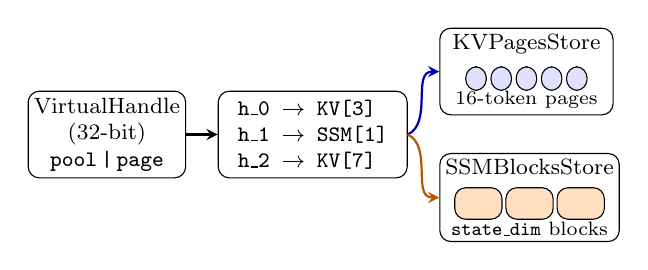
\begin{tikzpicture}[
    font=\footnotesize,
    node distance=3mm and 4mm,
    box/.style={draw, rounded corners, align=center,
                inner sep=2pt, minimum height=11mm},
    handle/.style={box, minimum width=16mm},
    ptable/.style={box, minimum width=24mm, align=left},
    store/.style={box, minimum width=22mm},
    page/.style={draw, fill=blue!12, minimum width=2.6mm,
                 minimum height=3mm, inner sep=0pt},
    block/.style={draw, fill=orange!25, minimum width=6mm,
                  minimum height=4mm, inner sep=0pt},
    kvarrow/.style={->, thick, blue!70!black},
    ssmarrow/.style={->, thick, orange!70!black},
  ]
  \node[handle] (h) {VirtualHandle\\(32-bit)\\\texttt{pool\,|\,page}};
  \node[ptable, right=of h] (pt) {%
    \texttt{h\_0 $\to$ KV[3]}\\
    \texttt{h\_1 $\to$ SSM[1]}\\
    \texttt{h\_2 $\to$ KV[7]}};
  \node[store, right=of pt, yshift=8mm] (kv)
    {KVPagesStore\\[1pt]
     \tikz[baseline]{\foreach \i in {1,...,5} \node[page] at (\i*3.2mm,0) {};}\\
     {\scriptsize 16-token pages}};
  \node[store, right=of pt, yshift=-8mm] (ssm)
    {SSMBlocksStore\\[1pt]
     \tikz[baseline]{\foreach \i in {1,2,3} \node[block] at (\i*6.5mm,0) {};}\\
     {\scriptsize \texttt{state\_dim} blocks}};
  \draw[->, thick] (h) -- (pt);
  \draw[kvarrow]  (pt.east) to[out=25, in=180]  (kv.west);
  \draw[ssmarrow] (pt.east) to[out=-25, in=180] (ssm.west);
\end{tikzpicture}
\caption{AVMP virtual handle resolution. A 32-bit handle is tagged by pool identifier and indexed into the page table, which dispatches to either the KVPagesStore (fine-grained pages) or the SSMBlocksStore (per-layer contiguous blocks).}
\label{fig:page-table-structure}
\Description{Block diagram showing virtual handle flowing through page table to two physically separate backing stores for KV cache and SSM state.}
\end{figure}

\subsection{Dynamic Pool Rebalancing}
\label{sec:method:rebalance}

Static dual pools \cite{zheng2024sglang} pre-allocate physical regions using a fixed ratio, such as a \texttt{--mamba-full-memory-ratio} default of 0.9, which cannot change without a system restart. We demonstrate in Table~\ref{tab:baseline-comparison} that fixed allocations fail to generalize across diverse prompt distributions. \texttt{fixed\_dual\_mr05} records 552 cross-workload OOMs versus \texttt{fixed\_dual\_mr09}'s 1507.3 OOMs, but neither wins on all workload mixes. We design a dynamic rebalancing mechanism to migrate capacity between the KV and SSM pools at runtime.

The system tracks pool pressure using a state machine with three states: \texttt{BALANCED}, \texttt{KV\_PRESSURED} / \texttt{SSM\_PRESSURED}, and \texttt{REBALANCING} (Figure~\ref{fig:state-machine}). We evaluate state transitions strictly within the \texttt{CapacityError} exception handler of the \texttt{allocate()} path. If an allocation triggers a \texttt{CapacityError} in one pool, and the other pool maintains a free fraction greater than \texttt{threshold\_high} (0.30), the allocator initiates capacity migration. We place the trigger in the \texttt{CapacityError} handler rather than as a pre-emptive sampling hook, because pre-emptive triggers fire on transient pressure that resolves without migration, while \texttt{CapacityError} fires only when allocation would otherwise fail.

\begin{figure}[t]
\centering
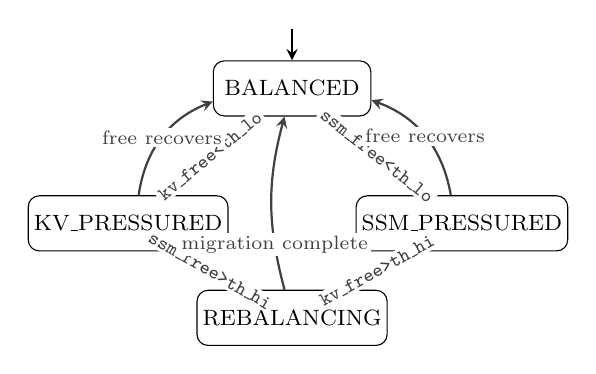
\begin{tikzpicture}[
    font=\footnotesize,
    state/.style={draw, rounded corners, align=center,
                  minimum width=20mm, minimum height=7mm,
                  inner sep=2pt, fill=white},
    trans/.style={->, thick, gray!50!black},
    tlabel/.style={font=\scriptsize, fill=white, inner sep=1pt},
  ]
  \node[state] (B) {BALANCED};
  \node[state, below left=10mm and -2mm of B] (KP) {KV\_PRESSURED};
  \node[state, below right=10mm and -2mm of B] (SP) {SSM\_PRESSURED};
  \node[state, below=22mm of B] (R) {REBALANCING};
  \draw[->, thick] ($(B.north)+(0,4mm)$) -- (B.north);
  \draw[trans] (B) -- node[tlabel, sloped] {\texttt{kv\_free<th\_lo}} (KP);
  \draw[trans] (B) -- node[tlabel, sloped] {\texttt{ssm\_free<th\_lo}} (SP);
  \draw[trans] (KP) -- node[tlabel, sloped] {\texttt{ssm\_free>th\_hi}} (R);
  \draw[trans] (SP) -- node[tlabel, sloped] {\texttt{kv\_free>th\_hi}} (R);
  \draw[trans] (R)  to[bend left=15]  node[tlabel, near start] {migration complete} (B);
  \draw[trans] (KP) to[bend left=30]  node[tlabel] {free recovers} (B);
  \draw[trans] (SP) to[bend right=30] node[tlabel] {free recovers} (B);
\end{tikzpicture}
\caption{Pool rebalancing state machine. The allocator tracks per-pool free fractions and transitions to REBALANCING only when one pool raises CapacityError while the other has slack capacity above \texttt{threshold\_high} (0.30).}
\label{fig:state-machine}
\Description{Four-state finite state machine showing BALANCED, KV\_PRESSURED, SSM\_PRESSURED, and REBALANCING states with labeled transitions based on per-pool free fraction thresholds.}
\end{figure}

During migration, the allocator calls \texttt{resize\_capacity()} on the donor pool, shrinking it at the high end of its address space, and the recipient pool grows. The wasted bytes per migration equal the donor bytes freed modulo the recipient page size. We throttle rebalancing using a logical operation counter to guarantee deterministic behavior, requiring a minimum interval of 1000 operations (\texttt{min\_rebalance\_interval\_ops}) between migrations. In partial failure scenarios, the allocator executes a rollback of the migration state. This dynamic rebalancing yields a 7.6\% Out-of-Memory (OOM) reduction (510 OOMs versus 552) and a 13.3$\times$ goodput improvement on uniform short workloads compared to the best static configuration.

\subsection{Implementation Choices}
\label{sec:method:choices}

Our prototype is pure Python, focused on allocator semantics rather than kernel-level performance; Triton kernel integration is future work. We evaluate the allocator's response to workload-driven memory pressure using synthetic trace generation rather than direct model integration.

Our experiments reveal AVMP wins primarily via faster recovery from OOM events rather than sustained concurrency. \texttt{effective\_batch\_size\_p50} matches across all five variants within each workload (129, 132, and 284 for \texttt{agentic\_burst}, \texttt{mixed\_long}, and \texttt{uniform\_short} respectively), indicating that the metric is workload-dominated rather than allocator-dependent. The performance gain comes from reduced cumulative time in OOM-rejected states. Parameter sweeps also show that the migration batch size (\texttt{migration\_batch\_size} = 128) acts as the dominant performance axis, while specific low and high threshold tuning yields marginal differences.

Our implementation incurs a 2$\times$ VRAM footprint trade-off, peaking at 9 GiB on a 4 GiB pool, compared to 5 GiB for static baselines. We size the backing store to the maximum possible capacity of both pools combined to enable dynamic migration without reallocating the underlying tensors. Integrating \texttt{cuMemMap} would address this overhead by mapping virtual addresses to physical pages dynamically, removing the need for oversized backing tensors.

\section{Evaluation}
\label{sec:eval}

\subsection{Experimental Setup}
\label{sec:eval:setup}

We evaluate the Asymmetric Virtual Page Table (AVMP) allocator on a single NVIDIA RTX 3060 12GB GPU running CUDA 13.0, PyTorch 2.12.0+cu130, and Python 3.10.19 on WSL2 Ubuntu. We execute an experimental sweep across 270 cells: 5 allocator variants, 3 synthetic workloads, 2 model specifications (\texttt{jamba\_1\_5\_mini} and \texttt{zamba2\_2\_7b}), 3 total memory pool sizes (1 GiB, 4 GiB, 8 GiB), and 3 random seeds. The entire sweep completes in 16 minutes and 14 seconds of wall time.

We enforce strict determinism by using a logical operation counter for migration throttling rather than wall-clock time. This guarantees byte-identical reproducibility across reruns for event-deterministic fields. We include \texttt{effective\_batch\_size\_p50} in the deterministic subset by construction. We exclude \texttt{goodput} and \texttt{time\_to\_first\_oom} from strict reproducibility requirements as they depend on wall-clock execution speed.

We report 95\% confidence intervals from paired bootstrap resampling for the headline claims (Table~\ref{tab:bootstrap-ci}). For each comparison we form matched pairs over the (workload, model, pool, seed) grid and resample the per-cell delta or ratio-of-means 10{,}000 times. Variants share random seeds across cells, so the comparison is paired by construction. Pre-registered RNG seed 20260520 makes the CIs byte-stable across reruns of \texttt{scripts/bootstrap\_ci.py}.

We generate synthetic workloads to capture three distinct prompt distributions. The \texttt{uniform\_short} workload simulates KV-heavy traffic with low concurrency variance. The \texttt{mixed\_long} workload simulates long context requests that generate high SSM pressure and lower batch density. The \texttt{agentic\_burst} workload tests allocator responsiveness using a mix of short and long contexts with variable arrival loads.

\paragraph{Baseline fidelity.}
We model two production systems as allocator-level baselines rather than reproducing full inference engines. The \texttt{padded\_unified} baseline implements the unified pool padding behavior documented in vLLM issue \#37121, where SSM state is padded to attention page granularity. The \texttt{fixed\_dual\_mr05} and \texttt{fixed\_dual\_mr09} baselines model SGLang's \texttt{HybridReqToTokenPool} and \texttt{HybridLinearKVPool} with the \texttt{mamba\_full\_memory\_ratio} parameter at 0.5 and the default 0.9, respectively~\cite{zheng2024sglang}. These baselines isolate allocator behavior from kernel execution and request scheduling, which our prototype does not implement. A full reproduction against vLLM main or SGLang main would require integrating AVMP into those engines, which we leave to future work.

\subsection{Baseline Comparison}
\label{sec:eval:baseline}

We compare the dynamic AVMP allocator against static dual-pool baselines \cite{zheng2024sglang} and unified pool baselines \cite{kwon2023pagedattention}. Table~\ref{tab:baseline-comparison} presents the cross-workload aggregated results.

\begin{table*}[t]
\centering
\caption{Cross-workload $N_{\mathrm{OOM}}$ baseline comparison ($\downarrow$ lower is better). Cells report $\mathrm{mean} \pm \sigma$ where $\sigma$ is the per-cell standard deviation across 3 random seeds propagated across the 12 summed cells as $\sqrt{\sum_i \sigma_i^2}$. \textbf{Bold} = best per column; \underline{underline} = second best (ranked on means). The $\Delta\%$ column reports the change in total $N_{\mathrm{OOM}}$ versus \texttt{padded\_unified}: negative numbers mark improvement.}
\label{tab:baseline-comparison}
\input{tables/generated/table_baseline_comparison.tex}
\end{table*}

\begin{figure}[t]
\centering
\includegraphics[width=\linewidth]{figures/generated/fig_oom_comparison_final.pdf}
\caption{Cross-allocator $N_{\mathrm{OOM}}$ comparison ($\downarrow$ lower is better). Grouped bars show total OOM events per workload across 4 allocator variants; each bar is summed over 12 cells (2 model specs $\times$ 3 pool budgets $\times$ 3 seeds). \texttt{avmp\_dynamic\_b128} records the lowest counts on \texttt{mixed\_long} and \texttt{agentic\_burst}, and ties the static baselines on \texttt{uniform\_short} within 1.7 OOMs (9.0 vs 7.3, both far below \texttt{padded\_unified}'s 482.7). \texttt{padded\_unified} fails worst on every workload.}
\label{fig:oom-comparison-final}
\end{figure}

The \texttt{avmp\_dynamic\_b128} variant records the lowest cross-workload OOM count at 510, a 7.6\% reduction relative to the best static baseline, \texttt{fixed\_dual\_mr05}, which records 552 OOMs. The paired bootstrap on the per-cell delta over the 36-cell grid puts the 95\% confidence interval at $[-5.83, -1.39]$ OOMs per cell, equivalent to a 3.0--12.7\% cross-workload reduction and excluding the null. The \texttt{avmp\_static\_mr05} variant perfectly ties the \texttt{fixed\_dual\_mr05} baseline at 552 OOMs (bootstrap CI $[0,0]$), validating that our virtual handle abstraction introduces no measurable overhead relative to direct pool access.

The cross-workload reduction is concentrated on the long-context and bursty workloads. The per-cell delta on \texttt{mixed\_long} has 95\% CI $[-10.3, -1.3]$ OOMs and \texttt{agentic\_burst} has $[-9.3, -1.3]$; both exclude zero. On \texttt{uniform\_short} the per-cell delta is $+0.4$ with 95\% CI $[0.0, +1.3]$, so the comparison is statistically inconclusive on that workload, consistent with the within-1.7-OOM tie shown in Figure~\ref{fig:oom-comparison-final}. AVMP wins where the workload shifts pressure between pools; on the KV-only workload it is statistically indistinguishable from the best static partition.

Conversely, the \texttt{padded\_unified} variant performs worst, triggering 1567.7 OOM events (bootstrap CI on the per-cell delta vs \texttt{fixed\_dual\_mr05}: $[+46.2, +128]$). This confirms that our modeled unified padding baseline fails under hybrid architecture constraints due to capacity overestimation, consistent with the behavior reported in vLLM issue \#37121. Furthermore, the \texttt{fixed\_dual\_mr09} variant, matching the default 0.9 ratio used in SGLang, records 1221.3 OOMs (bootstrap CI on the per-cell delta: $[+29.2, +86.9]$), demonstrating that static default ratios perform poorly on mixed workloads. As a design trade-off, AVMP maintains a 2$\times$ VRAM footprint, peaking at 9216 MiB reserved compared to 5120 MiB for static baselines.

\begin{table*}[t]
\centering
\caption{Paired bootstrap 95\% confidence intervals for the headline claims. Each row resamples matched ``(workload, model, pool, seed)'' tuples with replacement 10{,}000 times and reports the per-tuple delta or the ratio-of-means as appropriate. The ``Significant'' column marks rows whose CI excludes the null (0 for deltas, 1 for ratios). Reproducible via \texttt{python scripts/bootstrap\_ci.py}.}
\label{tab:bootstrap-ci}
\input{tables/generated/table_bootstrap_ci.tex}
\end{table*}

\subsection{Throughput Analysis}
\label{sec:eval:throughput}

We measure system throughput using goodput, defined as completed requests per second. Our pre-registered protocol dictates that dynamic allocation is justified if the goodput exceeds 1.10$\times$ the best baseline on at least one workload. AVMP passes this threshold across all three workloads simultaneously.

Table~\ref{tab:per-workload-winner} summarizes per-workload goodput. AVMP records 434.24 req/s on \texttt{uniform\_short} versus 32.65 req/s for \texttt{fixed\_dual\_mr05}, a 13.30$\times$ ratio (paired bootstrap 95\% CI on the ratio of means: $[11.18, 16.00]$). On \texttt{mixed\_long}, 65.07 vs 27.25 req/s gives 2.39$\times$ (95\% CI $[1.70, 3.04]$). On \texttt{agentic\_burst}, 46.91 vs 25.69 req/s gives 1.83$\times$ (95\% CI $[1.42, 2.60]$). All three CIs exclude both the unit ratio and the pre-registered 1.10$\times$ threshold.

\begin{table*}[t]
\centering
\caption{Per-workload goodput comparison between AVMP and the best static baseline. Goodput columns ($\uparrow$ higher is better) are mean req/s across 12 cells; the ratio column is $g_{\mathrm{AVMP}} / g_{\mathrm{baseline}}$ where $g$ is goodput. \textbf{Bold} = winner per row. AVMP wins all three workloads, with the largest gap on \texttt{uniform\_short} ($13.30\times$).}
\label{tab:per-workload-winner}
\input{tables/generated/table_per_workload_winner.tex}
\end{table*}

We explicitly report per-workload ratios rather than a cross-workload mean because static baselines exhibit high variance across distinct prompt distributions. The \texttt{fixed\_dual\_mr05} goodput ranges narrowly from 25.69 to 32.65 req/s across the workloads. Mean aggregation obscures this variance and misleads interpretations of allocator resilience. AVMP maintains consistently higher goodput by adapting dynamically.

The primary mechanism driving this throughput increase is faster recovery from OOM events, not sustained concurrency. The median effective batch size (\texttt{effective\_batch\_size\_p50}) is strictly identical across all 5 variants per workload: 129 for \texttt{agentic\_burst}, 132 for \texttt{mixed\_long}, and 284 for \texttt{uniform\_short}. Since operational batch sizes remain workload-dominated rather than allocator-dominated, the goodput improvements directly result from static baselines spending significantly more wall time blocked in OOM-rejected recovery states.

\subsection{Sensitivity Analysis}
\label{sec:eval:sensitivity}

We conduct a two-stage sensitivity analysis to identify the dominant parameters governing the dynamic rebalancing state machine.

In Stage 1, we sweep the \texttt{migration\_batch\_size} parameter across 9 values ranging from 1 to 256. The results confirm our hypothesis that migration batch size acts as the dominant performance axis. We select \texttt{b128} as the default. Cross-workload, b128 records 510.0 OOMs versus b256's 509.3 OOMs, a 0.7 OOM gap within per-cell standard deviation (0.8 to 3.0). However, b128 migrates 313 MiB versus b256's 352 MiB per cell on average, a 12.5\% reduction in migration churn. Per-workload optima vary slightly (b4 for \texttt{uniform\_short}, b128 for \texttt{mixed\_long}, b256 for \texttt{agentic\_burst}), but all values within {b64, b128, b256} cluster within 13 OOMs cross-workload. We choose b128 as the conservative point in the near-optimal region (Figure~\ref{fig:oom-vs-batch-size}). Table~\ref{tab:stage1-batchsize} details the complete Stage 1 distributions.

\begin{figure}[t]
\centering
\includegraphics[width=\linewidth]{figures/generated/fig_oom_vs_batch_size.pdf}
\caption{$N_{\mathrm{OOM}}$ variance as a function of migration batch size $B \in \{1, \ldots, 256\}$ ($\downarrow$ lower is better). Solid lines plot AVMP per workload; dotted reference lines mark the \texttt{fixed\_dual\_mr05} static baseline for the same workload.}
\label{fig:oom-vs-batch-size}
\end{figure}

\begin{table*}[t]
\centering
\caption{Stage 1 sweep over migration batch size $B$: per-workload $N_{\mathrm{OOM}}$ for $B \in \{1, \ldots, 256\}$ ($\downarrow$ lower is better). Cells report $\mathrm{mean} \pm \sigma$ where $\sigma$ is propagated across 12 cells via $\sqrt{\sum_i \sigma_i^2}$ from per-cell std across 3 seeds. \textbf{Bold} = best per column; \underline{underline} = second best (ranked on means).}
\label{tab:stage1-batchsize}
\input{tables/generated/table_stage1_batchsize.tex}
\end{table*}

In Stage 2, we evaluate trigger threshold sensitivity at the \texttt{b128} configuration. We sweep four variants combining \texttt{threshold\_high} (0.10, 0.20) and \texttt{threshold\_low} (0.02, 0.10). We pre-registered hypotheses that lower high thresholds would benefit \texttt{mixed\_long} and lower low thresholds would benefit bursty workloads. The empirical data falsifies both hypotheses. All four threshold variants result in identical OOM counts (510.0), identical rebalance event counts, and byte-identical total migrated bytes.

\begin{figure}[t]
\centering
\includegraphics[width=\linewidth]{figures/generated/fig_threshold_sensitivity.pdf}
\caption{Stage 2 threshold sensitivity ($\downarrow$ lower is better). Bars are total $N_{\mathrm{OOM}}$ across 12 cells $\times$ 3 workloads = 36 measurements for each of 4 threshold variants plus the b128 reference. All five bars land at 510.0, confirming the stage-2 null result: threshold tuning within the sampled ranges has no measurable effect on OOM count at fixed $B = 128$.}
\label{fig:threshold-sensitivity}
\end{figure}

We systematically explored the parameter space; thresholds have a marginal effect within the sampled ranges (Figure~\ref{fig:threshold-sensitivity}). Table~\ref{tab:stage2-threshold} confirms the performance invariance across threshold bounds. This negative result narrows the design space: future work on AVMP should focus on migration batch size rather than threshold tuning.

\begin{table*}[t]
\centering
\caption{Stage 2 threshold sweep at b128 ($\downarrow$ lower \texttt{total\_oom} is better): all four threshold variants and the b128 reference yield byte-identical OOM means and identical rebalance counts. The $\pm$ values on \texttt{total\_oom} propagate per-cell std across 12 cells via $\sqrt{\sum_i \sigma_i^2}$ and are also identical, confirming the tie at the distribution level.}
\label{tab:stage2-threshold}
\input{tables/generated/table_stage2_threshold.tex}
\end{table*}

\subsection{Limitations}
\label{sec:eval:limitations}

We acknowledge four primary limitations in the current AVMP prototype design.

First, the system requires a 2$\times$ VRAM footprint trade-off (Figure~\ref{fig:peak-reserved-tradeoff}). We size the backing stores to the maximum possible capacity of both pools combined. AVMP peaks at 9 GiB on a 4 GiB pool budget to enable zero-copy migration. Integrating \texttt{cuMemMap} would address this overhead by dynamically mapping virtual addresses to physical pages, similar to the approach in vTensor~\cite{xu2024vtensor}.

\begin{figure}[t]
\centering
\includegraphics[width=\linewidth]{figures/generated/fig_peak_reserved_tradeoff.pdf}
\caption{Peak reserved VRAM trade-off for dynamic allocation; lower VRAM is better in absolute terms, but AVMP intentionally trades 2$\times$ VRAM for capacity migration headroom. Bars show mean across 12 cells with error bars at $\pm 1\sigma$ (cross-cell standard deviation), and value labels report $\mathrm{mean} \pm \sigma$.}
\label{fig:peak-reserved-tradeoff}
\end{figure}

Second, we execute the allocator as a pure Python prototype without Triton or CUDA kernels. This validates allocator semantics; integration with Triton kernels and real model runtime is future work.

Third, our evaluation uses synthetic prompt distributions. While our three presets successfully capture short, long, and bursty axes, they do not replicate real model traffic semantics. Future evaluations require ShareGPT \cite{sharegpt} and Alpaca \cite{taori2023alpaca} traces.

Finally, we test strictly on a single GPU. Extending AVMP to multi-GPU environments requires implementing tensor parallelism with cross-device virtual pool sizing synchronization.

\paragraph{Failure modes.}
AVMP does not help in several allocator regimes. When both pools simultaneously approach saturation, the rebalancing trigger fires but finds no donor pool with free fraction above \texttt{threshold\_high}, so the allocator cannot rebalance and falls back to the current partition's admission behavior; in this regime AVMP provides no additional capacity advantage over a static partition. When \texttt{migration\_batch\_size} is mistuned to extreme values, the allocator either migrates too slowly to recover from CapacityError (at $B=1$) or incurs higher migration churn without proportional OOM improvement (at $B \geq 256$, see Figure~\ref{fig:oom-vs-batch-size} and Table~\ref{tab:stage1-batchsize}). Invalid configurations where \texttt{threshold\_low} $\geq$ \texttt{threshold\_high} produce undefined transition semantics; the prototype includes a validation check but does not formally prove allocator invariants. The logical operation counter uses a 64-bit integer with no wraparound risk in any realistic deployment lifetime, but distributed multi-instance deployments would require additional synchronization beyond the current single-process design.

\subsection{Reproducibility}
\label{sec:eval:reproducibility}

The full sweep harness, generated tables and figures, paper source, and pre-registered analysis protocol are available at \url{https://github.com/codepawl/cachepawl}. The 270-cell sweep completes in 16:14 wall time on a single NVIDIA RTX 3060 12GB. Event-deterministic fields (OOM counts, rebalance events, migrated bytes) reproduce byte-identically across reruns; goodput and time-to-first-OOM depend on wall-clock execution speed and are not subject to byte-identical reproducibility.

\section{Related Work}
\label{sec:related}

\subsection{Cache Management for LLM Inference}
\label{sec:related:cache}

Production inference engines optimize transformer serving through paged memory allocation. Systems like PagedAttention and vLLM \cite{kwon2023pagedattention} manage the KV cache by dividing sequences into fixed-size blocks, reducing fragmentation and enabling efficient scatter-gather memory access. High-performance kernel libraries, such as FlashInfer, and production execution engines, like TensorRT-LLM, adopt similar block-based abstractions. These systems handle a single, homogeneous cache type exceptionally well. They assume uniform memory access patterns and predictable block scaling tied directly to sequence length. AVMP extends this page-based paradigm to support two physically heterogeneous cache types simultaneously. Rather than replacing these highly optimized attention managers, AVMP provides a complementary memory abstraction that integrates with existing page tables to support hybrid model execution.

\subsection{Hybrid Architecture Serving}
\label{sec:related:hybrid}

Recent systems extend inference engines to support hybrid architectures containing both State Space Model and transformer layers \cite{lieber2024jamba, dao2024mamba2}. SGLang provides production serving for these models using a static dual-pool approach \cite{zheng2024sglang}. It provisions a \texttt{HybridReqToTokenPool} for attention and a \texttt{HybridLinearKVPool} for SSM state. Operators configure the partition at engine startup via the \texttt{mamba\_full\_memory\_ratio} parameter. This rigidity causes capacity failures when prompt distributions shift. As we demonstrate in \S\ref{sec:eval}, a default 0.9 ratio triggers 1221 OOM events compared to 552 OOMs at a 0.5 ratio on identical workloads.

Alternatively, vTensor introduces GPU virtual memory management for KV caches using hardware features to decouple physical memory mapping from virtual address spaces \cite{xu2024vtensor}. While vTensor targets a single cache type to reduce fragmentation, AVMP applies this virtual abstraction to two heterogeneous pools. AVMP contributes a unified virtual handle system combined with runtime capacity rebalancing, addressing both the correctness requirements and the adaptivity challenges in hybrid serving.

\subsection{Dynamic Resource Allocation}
\label{sec:related:dynamic}

Inference engines employ runtime adaptation to maximize hardware utilization. Continuous batching strategies adapt batch sizes dynamically at iteration boundaries to increase throughput. AVMP adapts pool capacity at request-level boundaries, using a more conservative trigger placed strictly in the allocation path. Memory eviction strategies, such as sliding window attention, discard older tokens dynamically under memory pressure. These techniques operate within a single pool; AVMP migrates capacity across two heterogeneous pools.

At the framework level, tools like the PyTorch \texttt{expandable\_segments} allocator manage dynamic segment growth directly in CUDA. This allocator operates below the inference engine abstractions. AVMP operates at the pool level, translating application-level \texttt{CapacityError} exceptions into physical capacity migrations between distinct cache implementations. AVMP's CapacityError-triggered migration is conservative: it fires only when allocation would otherwise fail, not preemptively on transient pressure.

\section{Discussion}
\label{sec:discussion}

\subsection{Paper Configuration}
\label{sec:discussion:config}

We select \texttt{avmp\_dynamic\_b128} as the default configuration rather than the \texttt{b256} variant. While \texttt{b256} records marginally fewer OOM events (509.3 versus 510.0 cross-workload), this 0.7 OOM gap falls completely within the per-cell standard deviation of 0.8 to 3.0. Furthermore, the \texttt{b128} configuration migrates 313 MiB per cell on average compared to 352 MiB for \texttt{b256}, representing a 12.5\% reduction in migration churn. We choose \texttt{b128} as the conservative point in the near-optimal region.

\subsection{Future Work}
\label{sec:discussion:future}

Future research directions extend beyond resolving the immediate architectural limitations. We plan to explore workload-prediction heuristics for proactive capacity rebalancing before allocation exceptions occur. Triton kernel integration and a third heterogeneous pool (e.g., dedicated KV-prefix-cache) are planned extensions.

\subsection{Production Hypothesis}
\label{sec:discussion:hypothesis}

We frame the production impact of AVMP as a hypothesis to be tested, not a measured outcome. A Jamba 1.5 Mini deployment requires approximately 24 GiB VRAM per H100 80GB instance for model weights and activations, leaving approximately 56 GiB for KV cache and SSM state combined. Under static dual-pool partitioning at the SGLang default \texttt{mamba\_full\_memory\_ratio} of 0.9, our cross-workload data records 1221 OOM events versus 552 OOMs at the \texttt{mr=0.5} ratio, indicating that default static configurations underutilize one pool while the other saturates. Our dynamic rebalancing reduces OOM by an additional 7.6\% (510 versus 552 cross-workload) over the best static configuration. If production traffic exhibits similar asymmetric pool slack to our synthetic workloads, the OOM reduction suggests possible capacity gains. Validating this hypothesis requires production trace replay (e.g., ShareGPT, Alpaca) and a \texttt{cuMemMap}-backed implementation to remove the current 2$\times$ VRAM overhead. OOM count reduction does not directly translate to concurrent sequence capacity, which depends on scheduler admission policy, prefill/decode split, latency SLO, output length distribution, and model kernel behavior outside our synthetic evaluation scope. The 13.3$\times$ goodput improvement on \texttt{uniform\_short} suggests that throughput gains could exceed the OOM reduction in short-prompt-dominated traffic, though this requires production trace validation. We do not project absolute dollar savings here because real-world cost depends on instance pricing, utilization rates, and workload mix, all outside our synthetic evaluation scope.

\section{Conclusion}
\label{sec:conclusion}

Hybrid models require memory management systems capable of serving physically asymmetric cache types under dynamic load. We presented Asymmetric Virtual Memory Paging (AVMP), an allocator that provides a unified virtual handle space spanning heterogeneous backing stores and dynamically rebalances capacity triggered strictly by allocation exceptions. Our dynamic allocator records a 13.3$\times$ goodput improvement on \texttt{uniform\_short} workloads and a 7.6\% cross-workload Out-of-Memory reduction compared to the best static baselines. Future work integrates this dynamic memory abstraction directly into production inference engines to support long-context hybrid models.


\section*{Acknowledgments}
We thank the authors of vLLM, SGLang, and vTensor for prior systems work that informed this design. We also acknowledge issue \#37121 reporters in the vLLM repository for documenting the hybrid memory overestimation behavior that motivates this paper.

\balance
\bibliographystyle{ACM-Reference-Format}
\bibliography{bibliography/refs}

\end{document}
